\documentclass[ignorenonframetext,t,10pt]{beamer}

\mode<presentation>
{ \usetheme{boxes} }


\usetheme[hideothersubsections]{UNLTheme}

%\usetheme{Warsaw}
%\usecolortheme{default}
%\useoutertheme{split}
%\useinnertheme{rectangles}
\definecolor{beamer@lblue}{rgb}{0.5,0.5,0.9}
\definecolor{beamer@dblue}{rgb}{0.1,0.1,0.5}
\setbeamercolor{structure}{fg=beamer@dblue}
%\beamertemplatenavigationsymbolsempty

% Language packages
\usepackage[english]{babel}
\usepackage[utf8]{inputenc}

% Packages
%%%%%%%%%%%%%%%%%%%%%%%%%%%%%%
% AMS packages
\usepackage{amsthm}
\usepackage{amsmath}
\usepackage{amsfonts}

% Images/figures
\usepackage{graphicx}
\usepackage{subfigure}

% Other
\usepackage{verbatim}
\usepackage{ifthen}
\usepackage{algorithmic}

\usepackage{epstopdf}

\usepackage{graphicx} %The mode "LaTeX => PDF" allows the following formats: .jpg  .png  .pdf  .mps
%\usepackage{media9}
\usepackage{movie15}

\usepackage{tikz}
\usetikzlibrary{shapes,arrows}

%%%%%%%%%%%%%%%%%%%%%%%%%%%%%%%

% Define some useful colors
\definecolor{tannerBlue}{rgb}{0.255,0.41,0.884} % RoyalBlue
\definecolor{tannerRed}{rgb}{1,0,0} % Red
% to use these colors: \textcolor{tannerBlue}{this text is blue}

% Commands
\newcommand{\tpvspace}{\vspace{5pt}}
\newcommand{\nicesum}{\displaystyle \sum}

%the following commands are used to align and insert slide numbers
\newcommand{\numspace}
{
  \ifthenelse{\insertframenumber < 10}{\hspace{30pt}}{\hspace{32pt}}
}
%\newcommand{\framenumbers}{\numspace\insertframenumber/{9}}

\newcommand{\pdfmovie}[4]{\href{run:#1}{\framebox{\parbox[c][#3][c]{#2}{\center #4}}}}


\pgfdeclareimage[height=1.0cm]{logo}{plots/caltech}
\logo{\pgfuseimage{logo}}

% Title
\title[Status of Seismon]{Status of Seismon}
\author[N.~Mukund, M.~Coughlin]{Nikhil Mukund, Michael Coughlin, Jan Harms, Nicolas Arnaud, David Barker, Sebastien Biscans, Eric Coughlin, Fred Donovan, Paul S Earle, Jeremy Fee, Irene Fiori, Hunter Gabbard, Michelle R Guy, Brian Lantz, Richard Mittleman, Arnaud Pele, Hugh Radkins, Bas Swinkels, Keith Thorne, Jim Warner}
\date[]{\today}

\begin{document}

\maketitle

\begin{frame}
\titlepage
\end{frame}

\section{Introduction}

\begin{frame}
\frametitle{Introduction}

  \begin{enumerate}
  \item The detectors are susceptible to teleseismic events, which can significantly impact a detector's duty cycle. 
  \item During O1 and O2, we used \emph{Seismon}, an early-warning system for gravitational-wave observatories, which relies on near real-time earthquake alerts provided by the U.S. Geological Survey (USGS) and the National Oceanic and Atmospheric Administration (NOAA).
  \item It had three methods for internal alert consumption: a Java applet written by Jan Harms (QuakeAlarm), a webpage designed by Hunter Gabbard (Terramon), and an EPICs client written by Keith Thorne and maintained by Sebastien Biscans, Jim Warner, and others.
  \end{enumerate}
\end{frame}

\section{Algorithm}

\begin{frame}
\frametitle{Pipeline}

% Define block styles
\tikzstyle{decision} = [diamond, draw, fill=blue!20,
    text width=4.5em, text badly centered, node distance=3cm, inner sep=0pt]
\tikzstyle{block} = [rectangle, draw, fill=blue!20,
    text width=5em, text centered, rounded corners, minimum height=3em]
\tikzstyle{line} = [draw, -latex']
\tikzstyle{cloud} = [draw, ellipse,fill=red!20, node distance=3cm,
    minimum height=2em]
\tikzstyle{emptyblock} = [rectangle, minimum height=3em]

\begin{figure}[t]
 \begin{center}
 \begin{tikzpicture}[node distance = 1.5cm, auto]
    % Place nodes
    \node [emptyblock] (init) {};
    \node [block, left of=init] (PDL) {PDL};
    \node [block, right of=init] (GeoJSON) {GeoJSON};
    \node [block, below of=init] (Parse) {Parse events};
    \node [block, below of=Parse] (Traveltimes) {Calculate travel times};
    \node [block, below of=Traveltimes] (XML) {Produce XML files};
    \node [block, below of=PDL, node distance=6cm] (Terramon) {Terramon};
    \node [block, below of=GeoJSON, node distance=6cm] (Epics) {Site Notification};
    % Draw edges
    \path [line] (PDL) -- (Parse);
    \path [line] (GeoJSON) -- (Parse);
    \path [line] (Parse) -- (Traveltimes);
    \path [line] (Traveltimes) -- (XML);
    \path [line] (XML) -- (Terramon);
    \path [line] (XML) -- (Epics);
 \end{tikzpicture}
 \end{center}
 \caption{A flow chart of the \emph{Seismon} pipeline. The USGS's Product Distribution Layer (PDL) and public GeoJSON earthquake files provide information used by \emph{Seismon} to compute estimated site arrival times and Rayleigh wave velocities.}
 \label{fig:flowchart}
\end{figure}
\end{frame}

\begin{frame}
\frametitle{Notices}

  \begin{enumerate}
\item Warning system relies on the most preliminary notices of earthquakes currently available generated by worldwide networks of seismometers. 
\item USGS provides preliminary estimates of the location providing latitude, longitude, and depth of each event.
\item These solutions are distributed through USGS's Product Distribution Layer (PDL), which has been configured to receive notifications for all located earthquakes worldwide. 
\item They are also available at the USGS website in JSON files (and other formats).
  \end{enumerate}
\end{frame}

\begin{frame}
\frametitle{Data products}

Time-of-arrival predictions
  \begin{enumerate}
  \item P- and S- wave estimates given by Python version of iaspei-tau, which is based on 1-D Earth model.
  \item R-wave estimates given by bounding box of [2, 5]\,km\,s, with best estimate at 3\,km/s. (Rana also used a CNN based on picks that him and students did which he thinks did a bit better for R-wave arrivals... student project?).
  \end{enumerate}

Peak ground velocity estimates
  \begin{enumerate}
\item Previously fit an empirical equation.
\item Now use a MLA using EQ parameters (discussed next) to make ground velocity predictions.
  \end{enumerate}
  
Lockloss predictions
  \begin{enumerate}
\item Uses a MLA based on EQ parameters and ground velocity predictions to make lockloss predictions.
  \end{enumerate}
  
\end{frame}

\section{MLA}

\begin{frame}
\frametitle{Data augmentation}

\begin{enumerate}
\item To improve the learning and prevent early stopping, we augment the data by artificially adding noise (or jitter) to the predictor and response variables in a controlled fashion. 
\item We employ \textbf{S}ynthetic \textbf{M}inority \textbf{O}versampling \textbf{TE}chnique (SMOTE) to augment the data 
\item The presence of noise enhances the ability of the MLA to better learn and generalize to the the underlying smooth nonlinear function. 
\item New samples are generated from each of the original dataset by creating a gaussian jitter distribution centered around the parameter value followed by random draw of samples from these distributions. 
\item Selective boosting is done so that the imbalances in the dataset are minimized. 
\end{enumerate}

\end{frame}

\begin{frame}
  \frametitle{Fit of peak velocities seen during O1-O2 at the interferometers.}
\begin{center}
\begin{figure}[hbtp!]
  \subfigure[Fit of peak velocities seen during O1-O2 at the interferometers (LHO and LLO) using Gaussian Process Regression. The events have been ordered by their measured peak ground velocity (in grey) and yellow error bar corresponds to a factor of 2 within the predicted value. About 90\% of events are within a factor of 2 of the predicted value.]{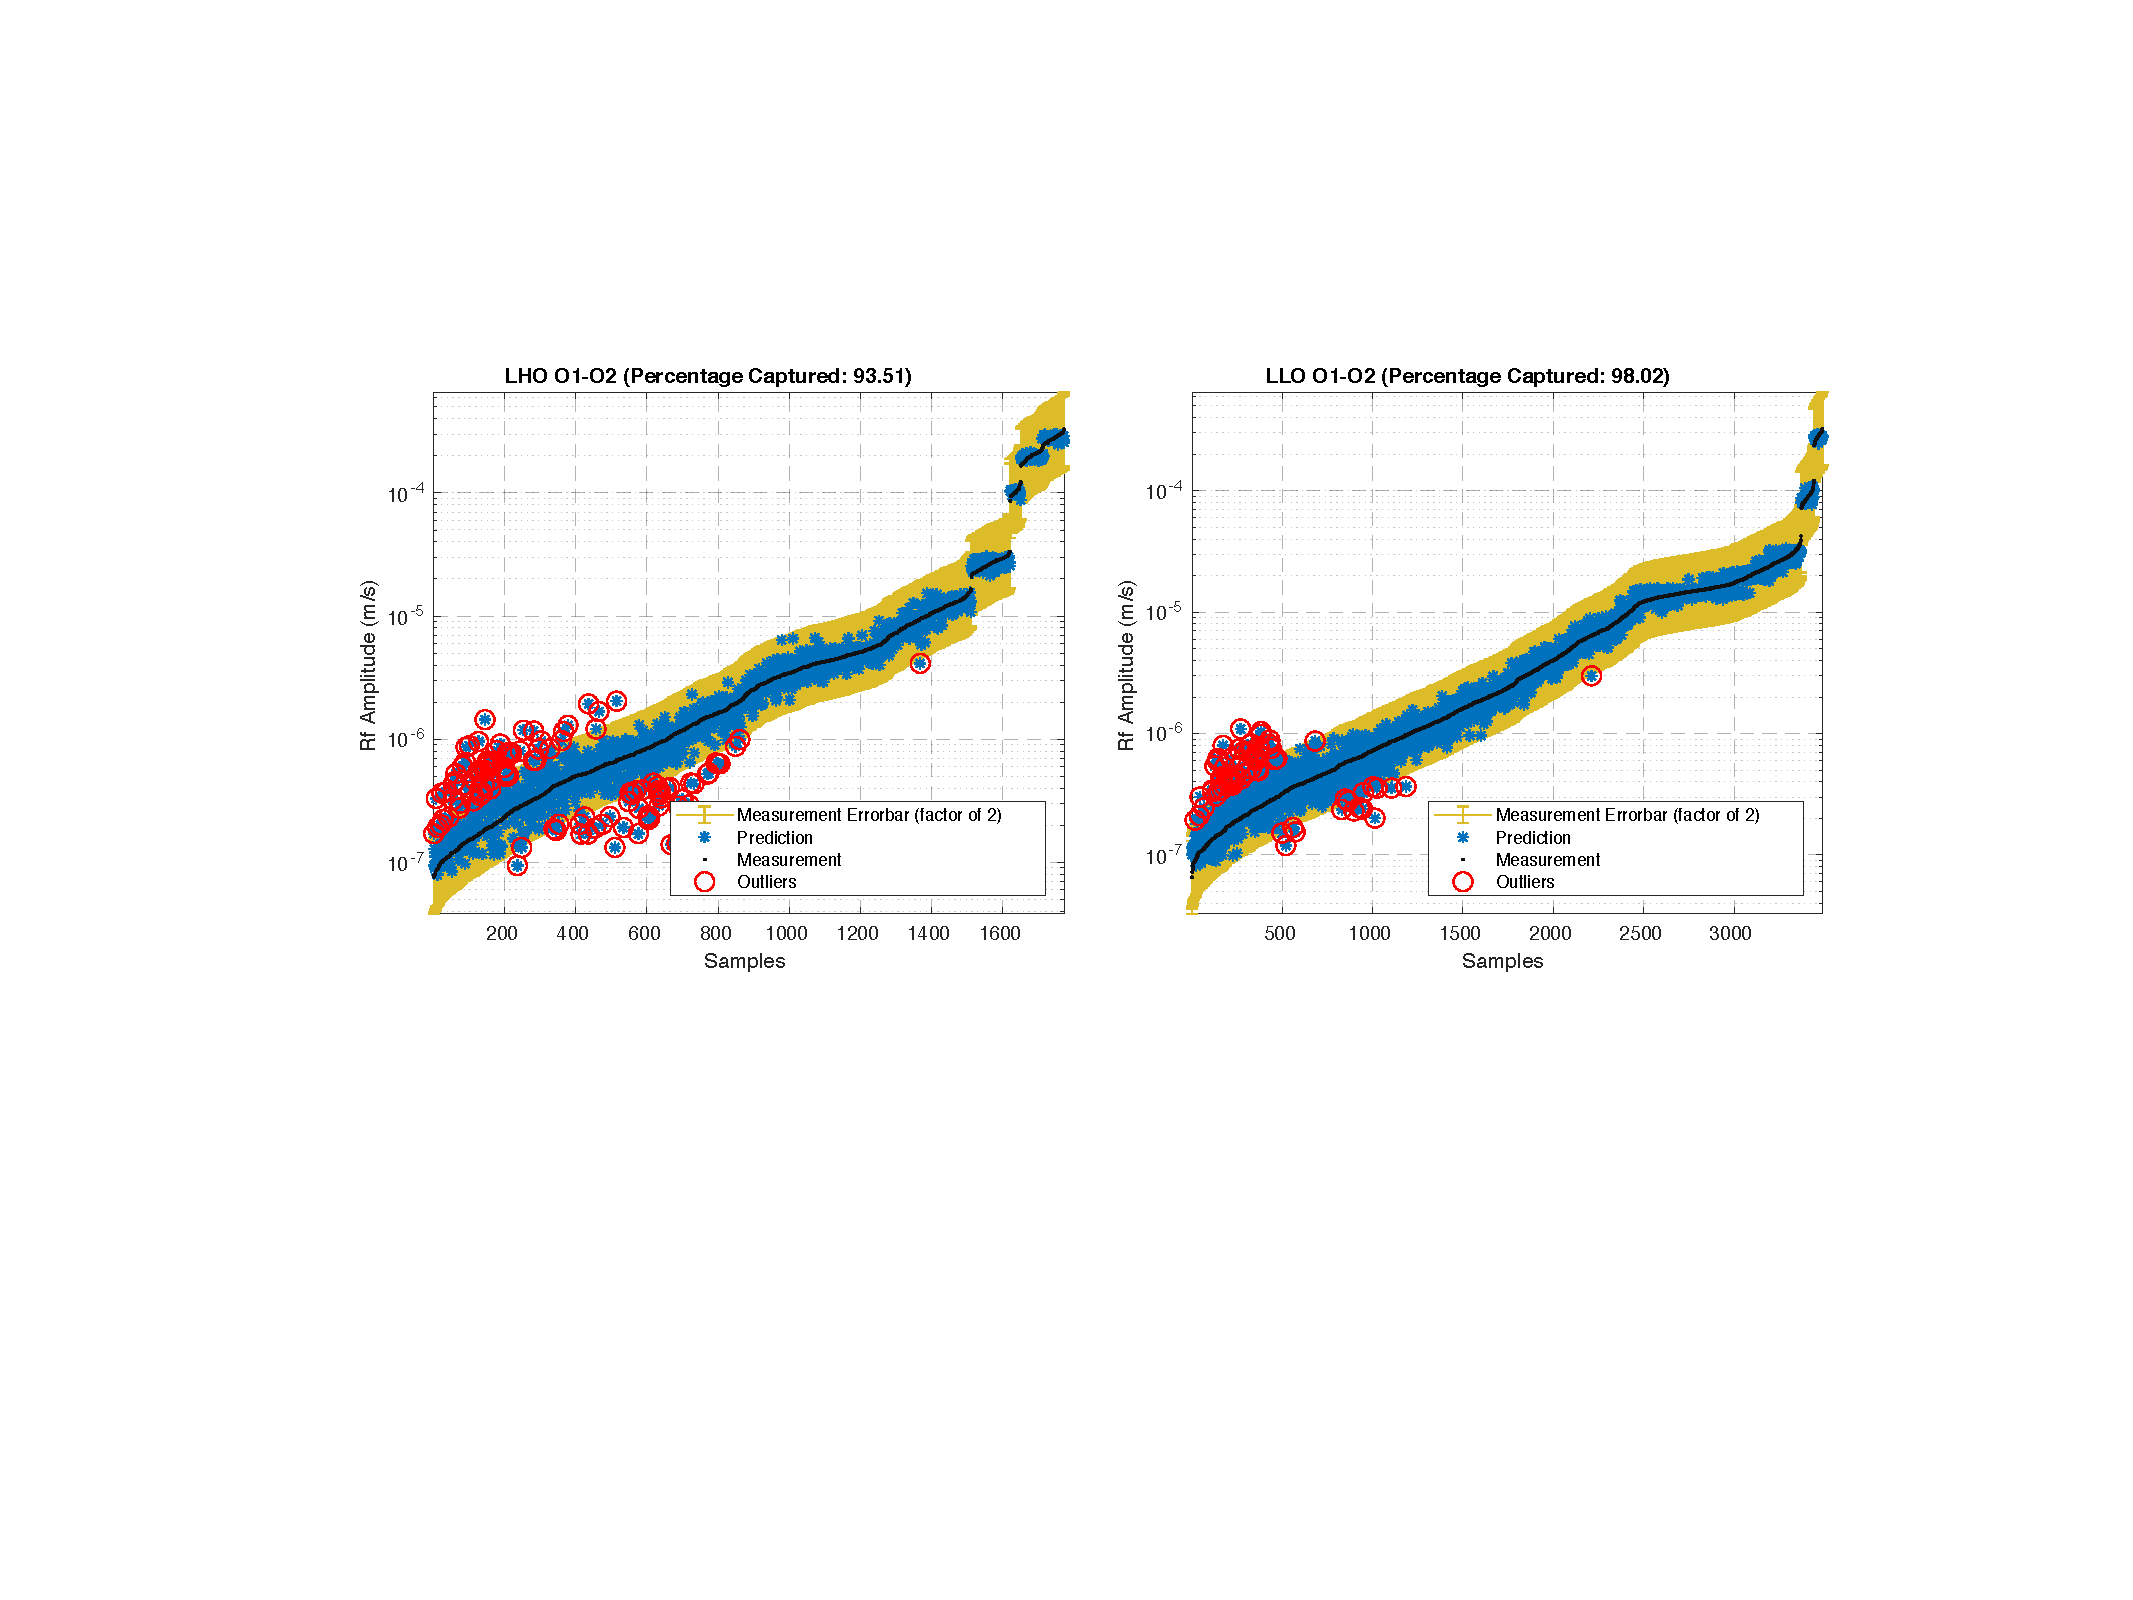
\includegraphics[trim = 0mm 0mm 1mm 0mm, clip = true, scale = 0.4]{plots/GPR_Matlab_O1O2.pdf}}
\end{figure}
\end{center}
\end{frame}

\begin{frame}
  \frametitle{Impact of earthquakes happening worldwide on gravitational-wave Inteferometers.}
\begin{center}
\begin{figure}[hbtp!]
  \subfigure[Impact of earthquakes happening worldwide on gravitational-wave Inteferometers.]{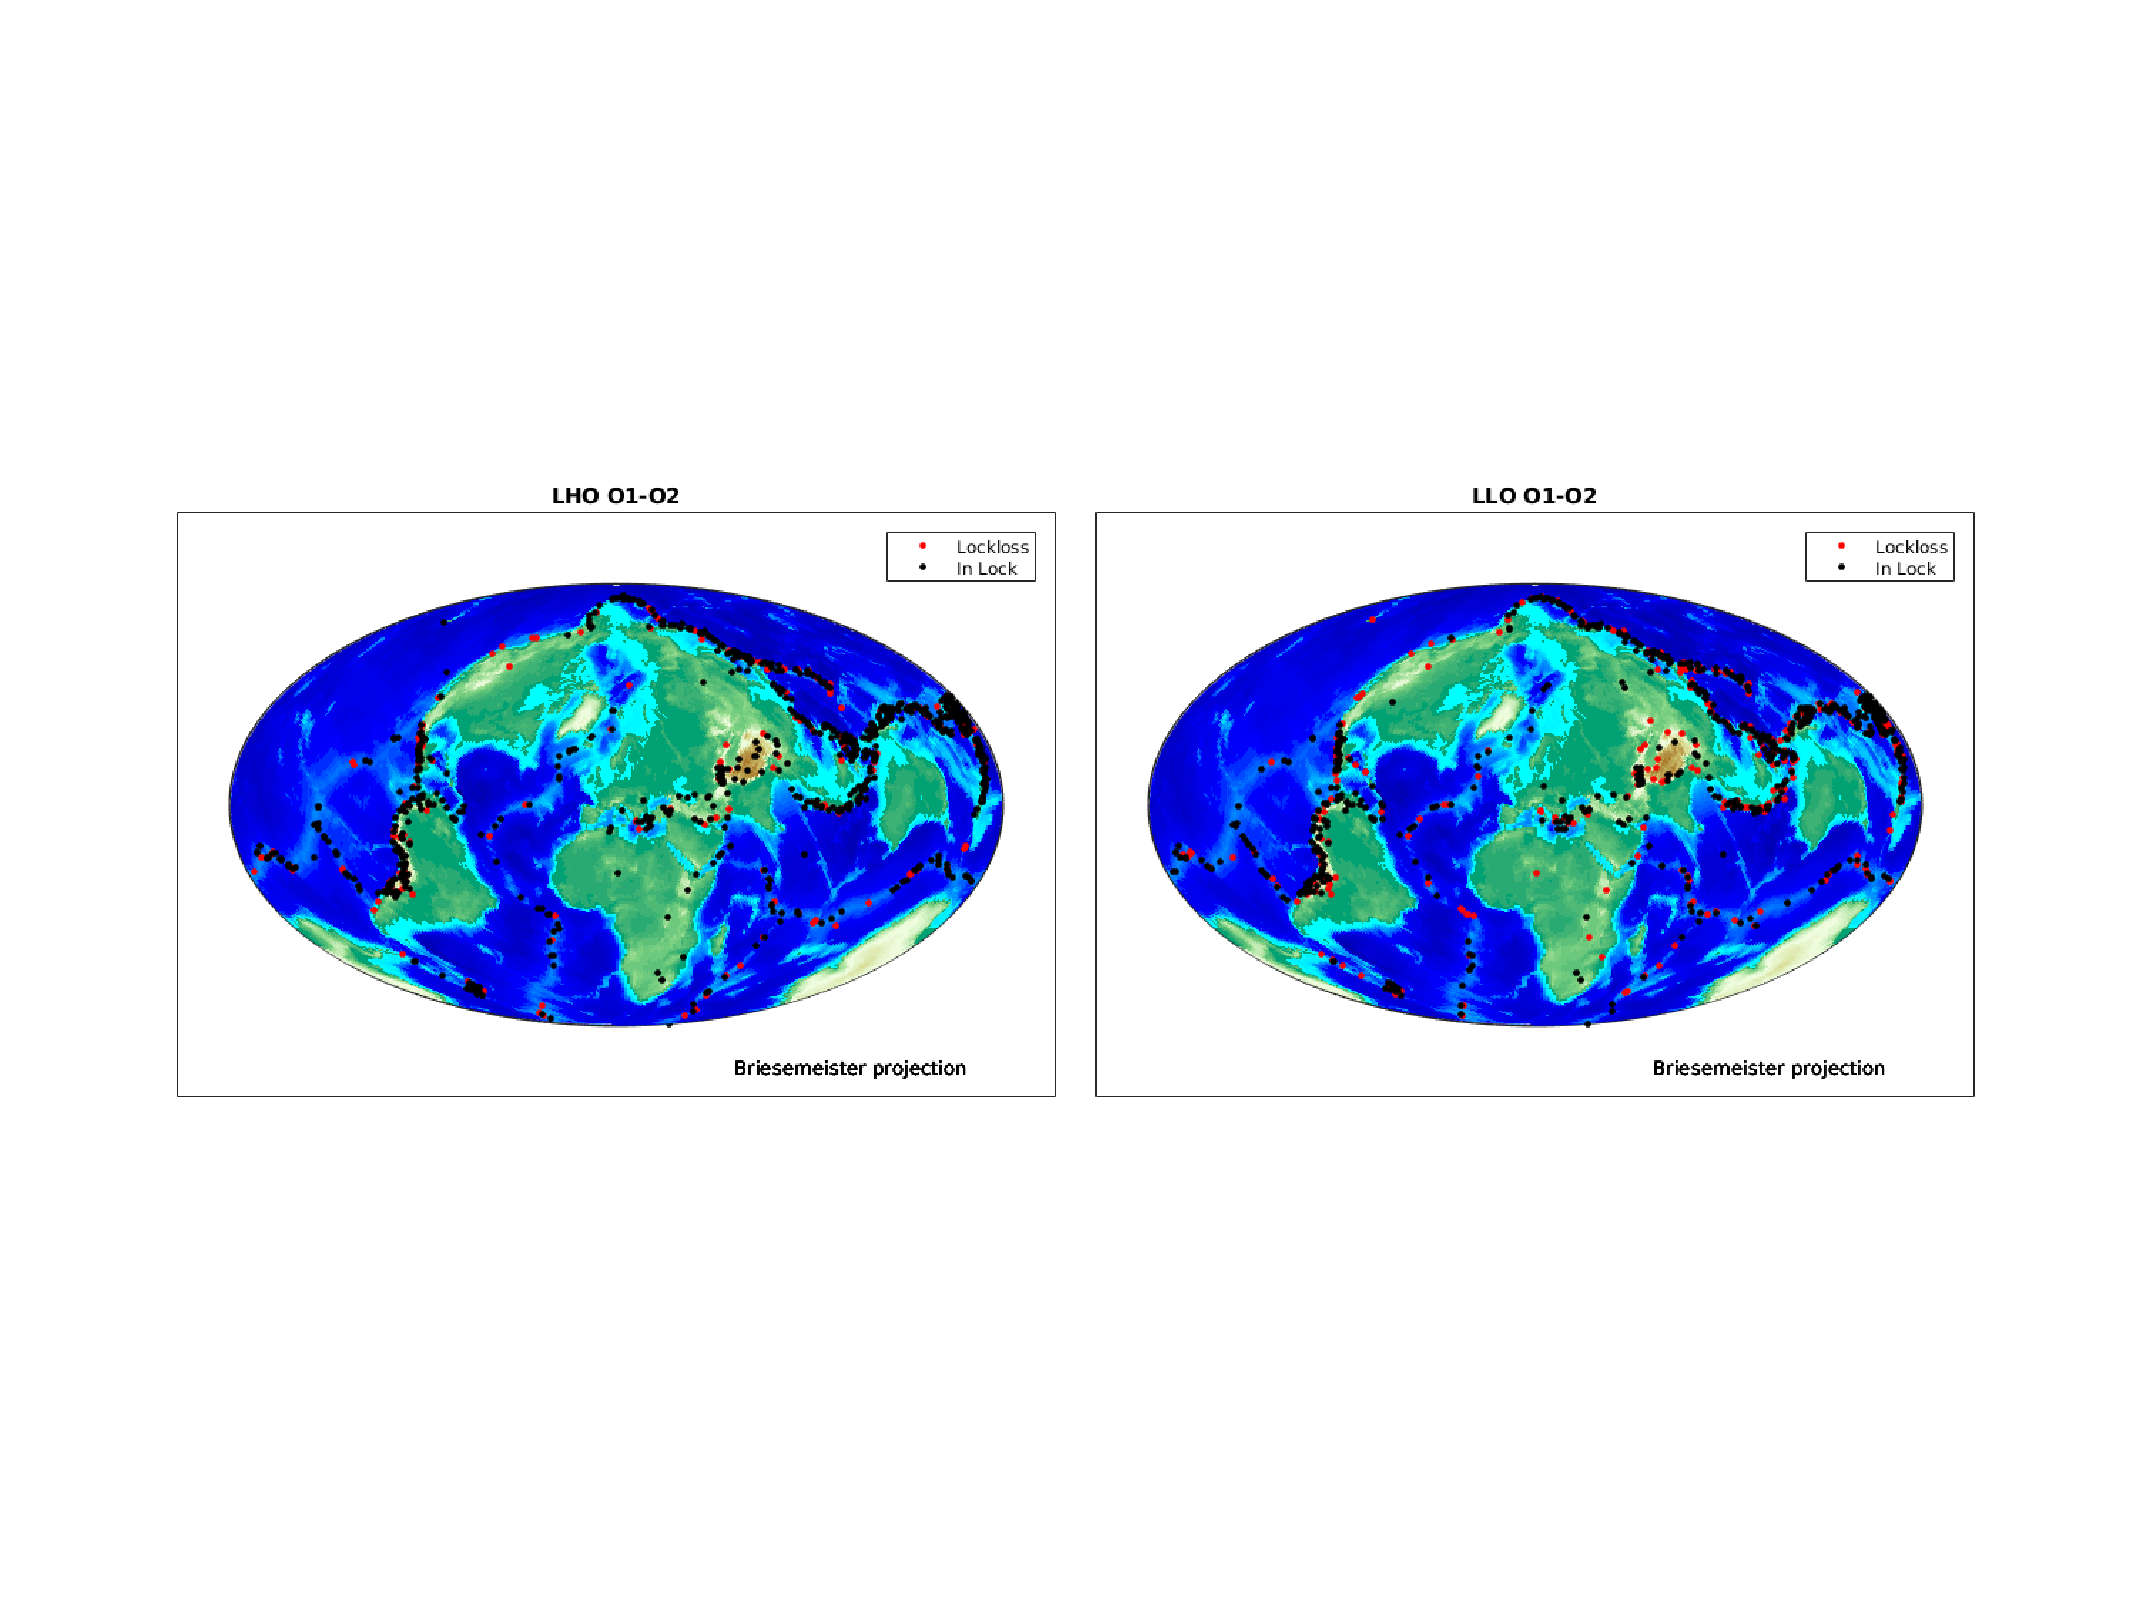
\includegraphics[trim = 0mm 0mm 1mm 0mm, clip = true, scale = 0.3]{plots/EQ_Distribution.pdf}}
\end{figure}
\end{center}
\end{frame}

\begin{frame}
  \frametitle{Performance of prediction at other sites.}
  
\begin{center}
\begin{figure}[hbtp!]
  \subfigure[The plot shows the location of seismic stations with available data from IRIS in the United States during the an earthquake. The color indicates the fractional error between the measured peak ground velocity and that predicted by the algorithm. The inset shows the location of the earthquake.]{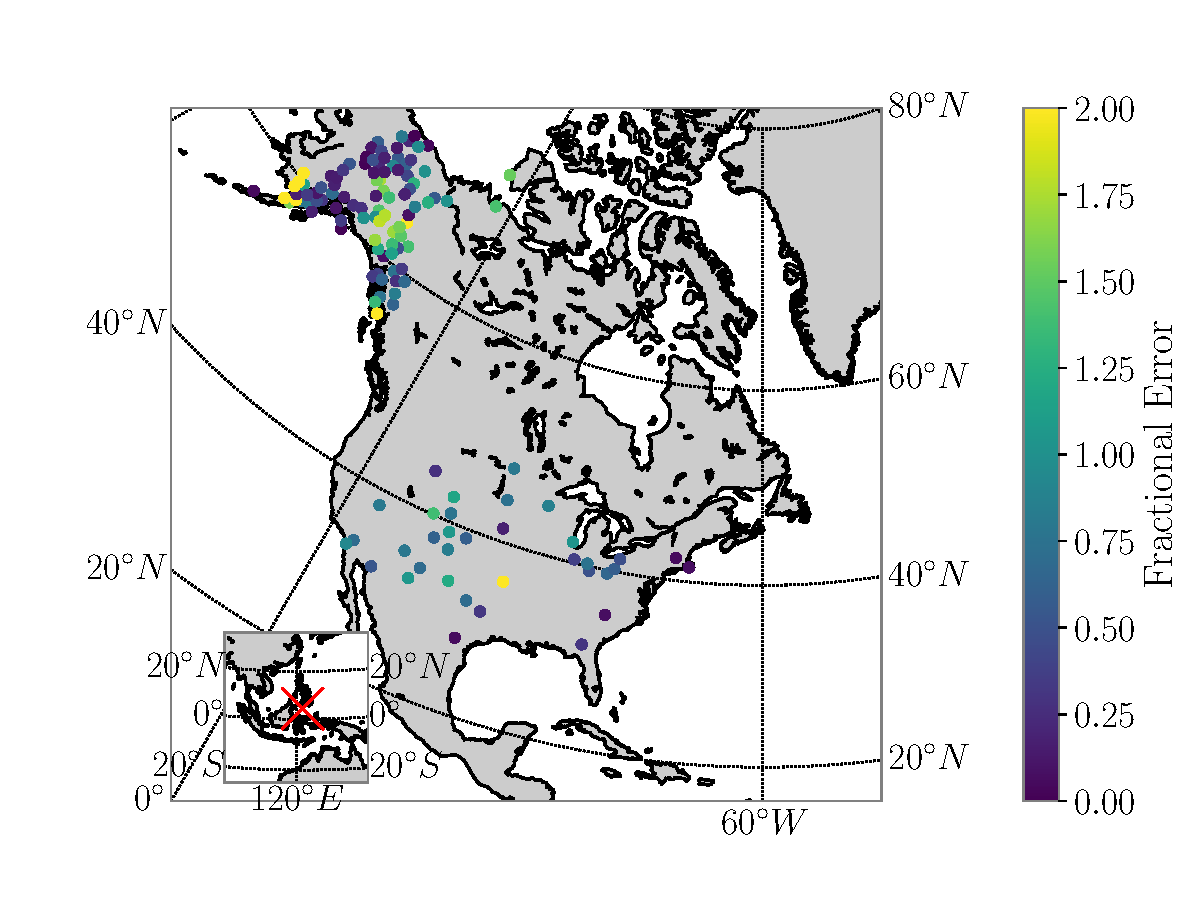
\includegraphics[trim = 0mm 0mm 1mm 0mm, clip = true, scale = 0.5]{plots/maps_vel_pred_vs_measured.pdf}}
\end{figure}
\end{center}
\end{frame}

\section{Conclusion}
\begin{frame}
  \frametitle{Conclusion}

In conclusion,
\begin{enumerate}
\item \emph{Seismon} is running reasonably well at LHO/LLO, with inputs to EPICs channels and the like. 
\item Virgo has installed and is running the code, and there is some debate about how to best use the output there.
\item Ability to do add fake earthquakes exists for testing.
\end{enumerate}

There is much to do going forward ...
\begin{enumerate}
\item Include updated ground velocity and lockloss predictions in \emph{Seismon}.
\item Install updated code at the sites (including the new LHO dedicated computer).
\item Use IRIS data to make global fits (and improve those at LHO, LLO, and Virgo?).
\item Control configuration changes
\end{enumerate}

\end{frame}

\section{Extra slides}

\end{document}
